\headline{{\textbf{\Large\sffamily Growing Together:}}\\
          {\textbf{\large\sffamily Bonsai Club News}}}
\label{2025-02-news}

% \topic{2025 Membership Renewal – Don't Forget!}
% \noindent
% Membership remains \textbf{£30} with monthly subs at \textbf{£5} for meetings at \emph{Whitton Community Centre} (extra sessions/external speaker nights may still incur additional costs). Payments can be made:
	
% \begin{itemize}
% 	\item \textbf{Online:} Twickenham Bonsai Club, A/C no. 53990897, Sort code 60-60-02 (please add a reference against the payment to help us identify where your payment has come from and log it via the Discord form as well).		
% 	\item \textbf{At the Next Meeting:} Cash or contactless.  
% \end{itemize}
	
% You can also prepay for the year's club nights—\textbf{12 sessions for £50 (10 months' price)}—bringing the total cost to \textbf{£80} for membership and subs.
	
\topic{Save on Club Merchandise with Shared Order!}
\noindent
The club's merchandise can be found at \url{https://overrock.uk/product-category/tw-bonsai/}. 
If you're thinking of making a purchase soon, reach out to Brendan on WhatsApp. 
Placing a shared order could help save a little on shipping costs.
	
\topic{Bonsai Insights: Information Pack for All Members}
\noindent
We've put together an information pack for all members of the club --- from beginners to seasoned enthusiasts. 
This pack offers a wealth of resources, including access to a selection of our lockdown ZOOM talks featuring some of the best Bonsai artists in the country.

The following link will direct you to a Google slideshow \href{https://docs.google.com/presentation/d/1L5SRA_ZSvnGMLbRt0CSf-Uz7BaiOfxOs7OUHMM_XrTY/edit?usp=sharing}{New \& Existing Members Information Pack}, so feel free to explore it at your own pace. 
We recommend starting with Andy Hardman's talk on tree biology (Video 1), where he delves into how trees function and what they need to thrive.

\topic{Don't Leaf Us Hanging: Meetup Time!}
\noindent
Come join us at 7pm on \textbf{13th March 2025} in the bar area at \emph{Whitton Community Centre, Percy Road, Whitton TW2 6JL}.
Branching out, the subject of next \textbf{Tree of the Month} display will be \textbf{Yamadori, urban or wild}---bring your best!
\closearticle

\hfill
\begin{center}
	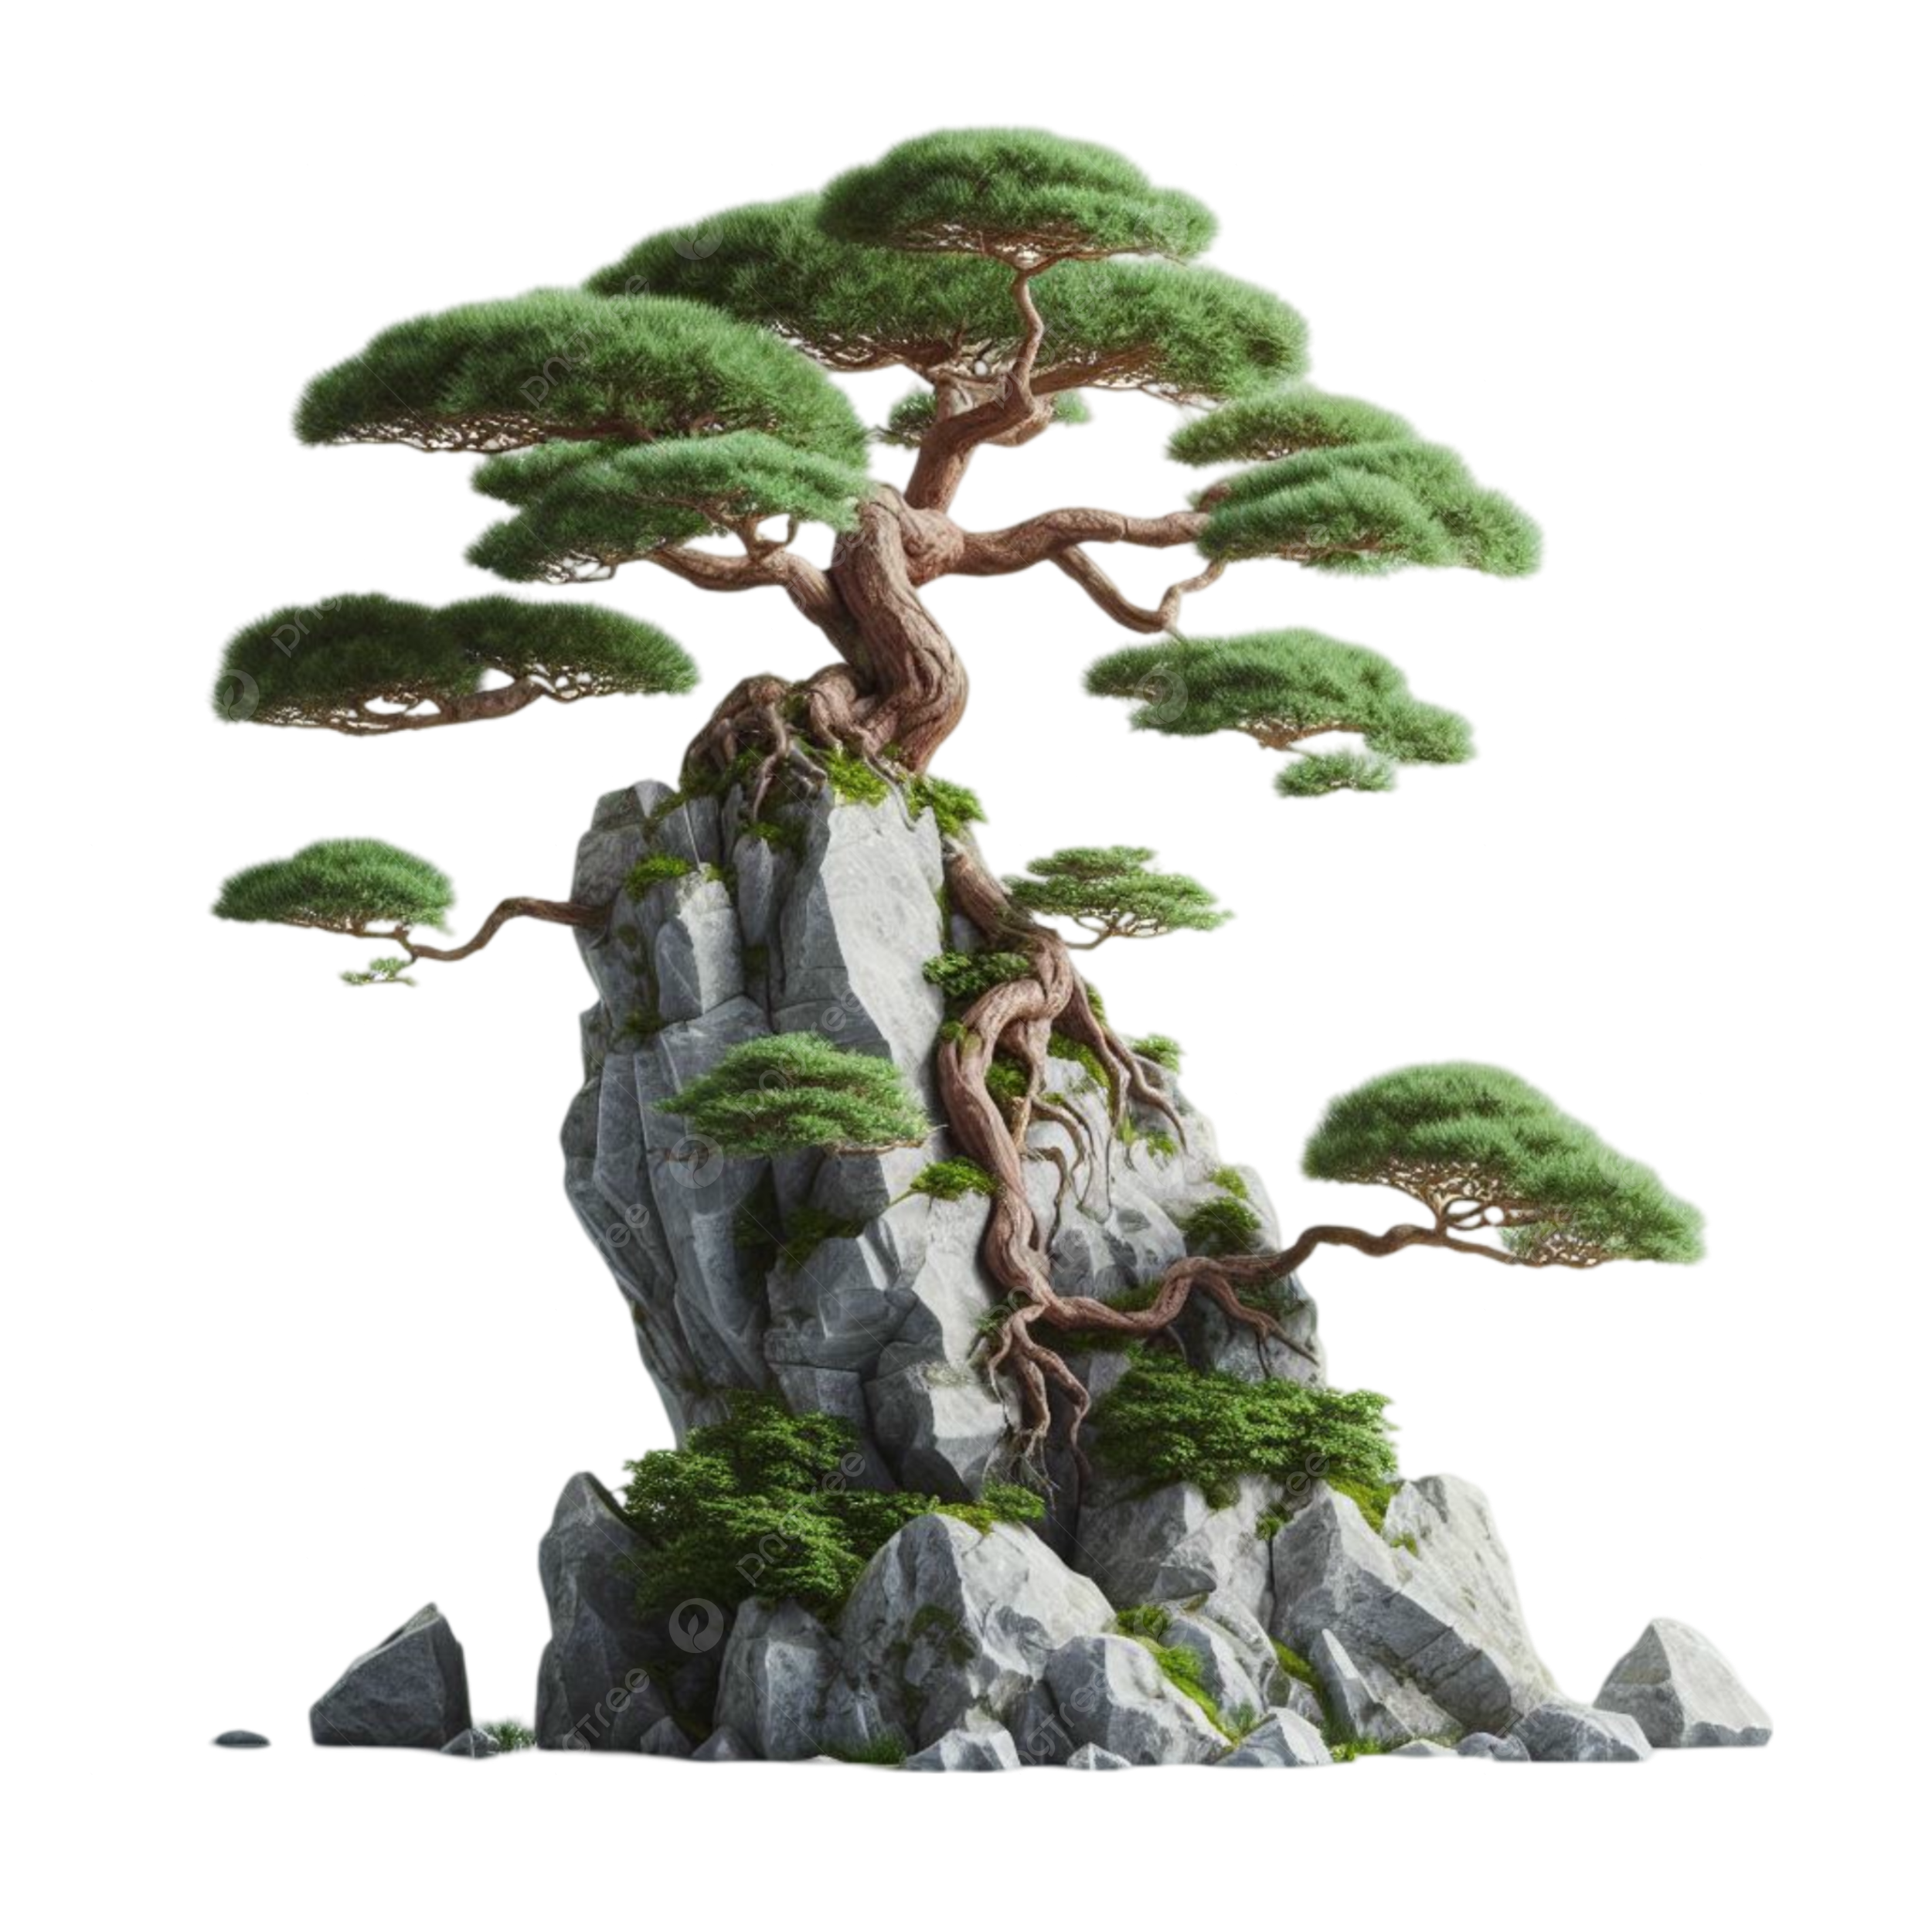
\includegraphics[width=0.8\columnwidth]{res/filler_d}
\end{center}

\columnbreak
